% Capítulo 2 - Fundamentação Teórica (versão enxuta): Emissão Acústica
Este capítulo apresenta os fundamentos necessários ao trabalho: a EA e a detecção de \textit{hits} (Seções~\ref{sec:UsoEA} e~\ref{sec:fund_hits}), o AM e as redes MLP (Seções~\ref{sec:AM} e~\ref{sec:MLP}) e os FPGAs, com as técnicas para executar modelos de AM nesses dispositivos (Seção~\ref{sec:FPGA}).

\section{Emissão Acústica na detecção de falhas}
\label{sec:UsoEA}

A EA é um método passivo de ensaio não destrutivo: eventos como trincas, erosão e o colapso de bolhas liberam energia de forma abrupta e geram ondas elásticas transitórias, captadas na superfície do equipamento por sensores piezoelétricos \cite{grosse2008acoustic,iso12716_2026}. Por registrar a atividade do próprio material em operação, a EA permite o monitoramento contínuo e não intrusivo e é sensível às fases iniciais da falha \cite{mba2006development}.

A Figura~\ref{fig:nde-ed-org-Fig1} mostra a cadeia de medição de um canal. O sensor converte a onda em um sinal elétrico da ordem de microvolts; um pré-amplificador eleva esse nível e, em geral, filtra a faixa de interesse, tipicamente de 100\,kHz a 1\,MHz; o sinal é então digitalizado por um conversor analógico-digital (\textit{Analog-to-Digital Converter}, ADC), a taxas de 1 a 40\,MSa/s, e processado para detectar eventos e calcular seus parâmetros \cite{grosse2008acoustic,vallen2022}.

\begin{figure}[htbp]
    \centering
    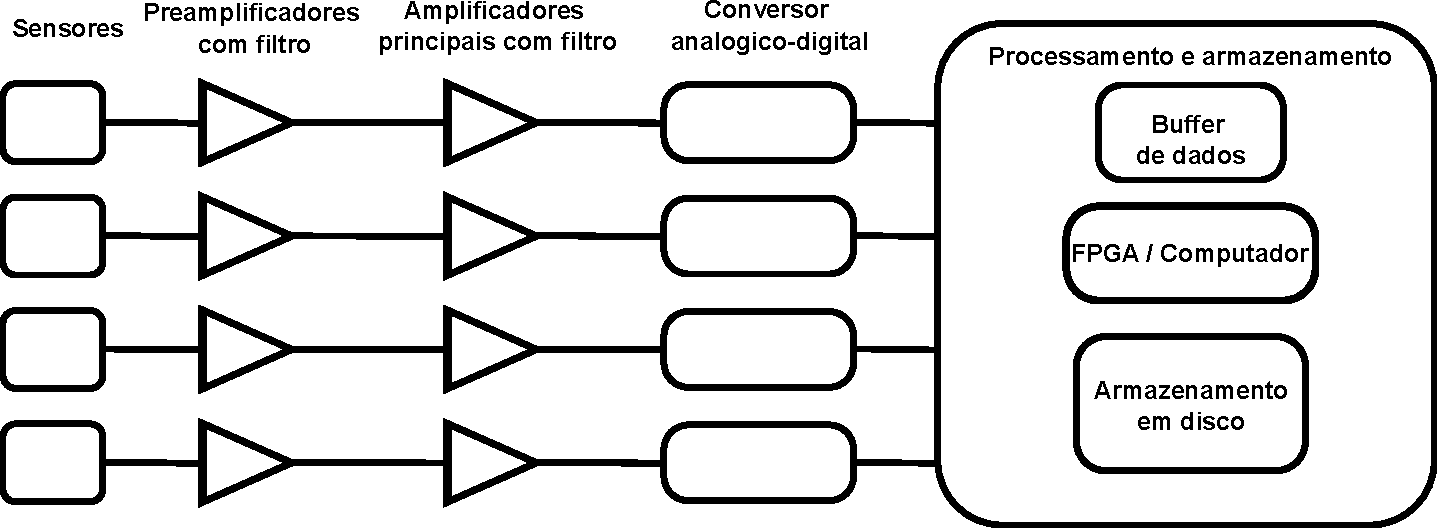
\includegraphics[width=.85\linewidth]{figs/Artigos/nde-ed-org/Figura1.pdf}
    \caption{Esquema funcional de um sistema de EA com sensores piezoelétricos, pré-amplificadores, filtros, amplificadores e aquisição digital. Adaptado de \citeonline{nde-ed-ae-equipment}.}
    \label{fig:nde-ed-org-Fig1}
\end{figure}

Um evento é registrado quando o sinal ultrapassa um \textbf{limiar} (\textit{threshold}) definido acima do ruído. Ele termina quando o sinal permanece abaixo do limiar por um intervalo pré-definido (\textit{hit definition time}, HDT, também chamado de DDT), e segue-se um tempo de bloqueio (\textit{hit lockout time}, HLT) em que novos cruzamentos não iniciam outro evento. Esse procedimento é a \textbf{detecção de \textit{hits}} (\textit{hit detection}), e o evento delimitado é um \textit{hit} \cite{vallen2022,unnthorsson2013}. De cada \textit{hit} extraem-se os parâmetros da Figura~\ref{fig:nde-ed-org-Fig2}: amplitude de pico, tempo de subida, duração, contagens de cruzamentos do limiar e energia. A definição operacional usada neste trabalho é detalhada na Seção~\ref{sec:fund_hits}.

\begin{figure}[htbp]
    \centering
    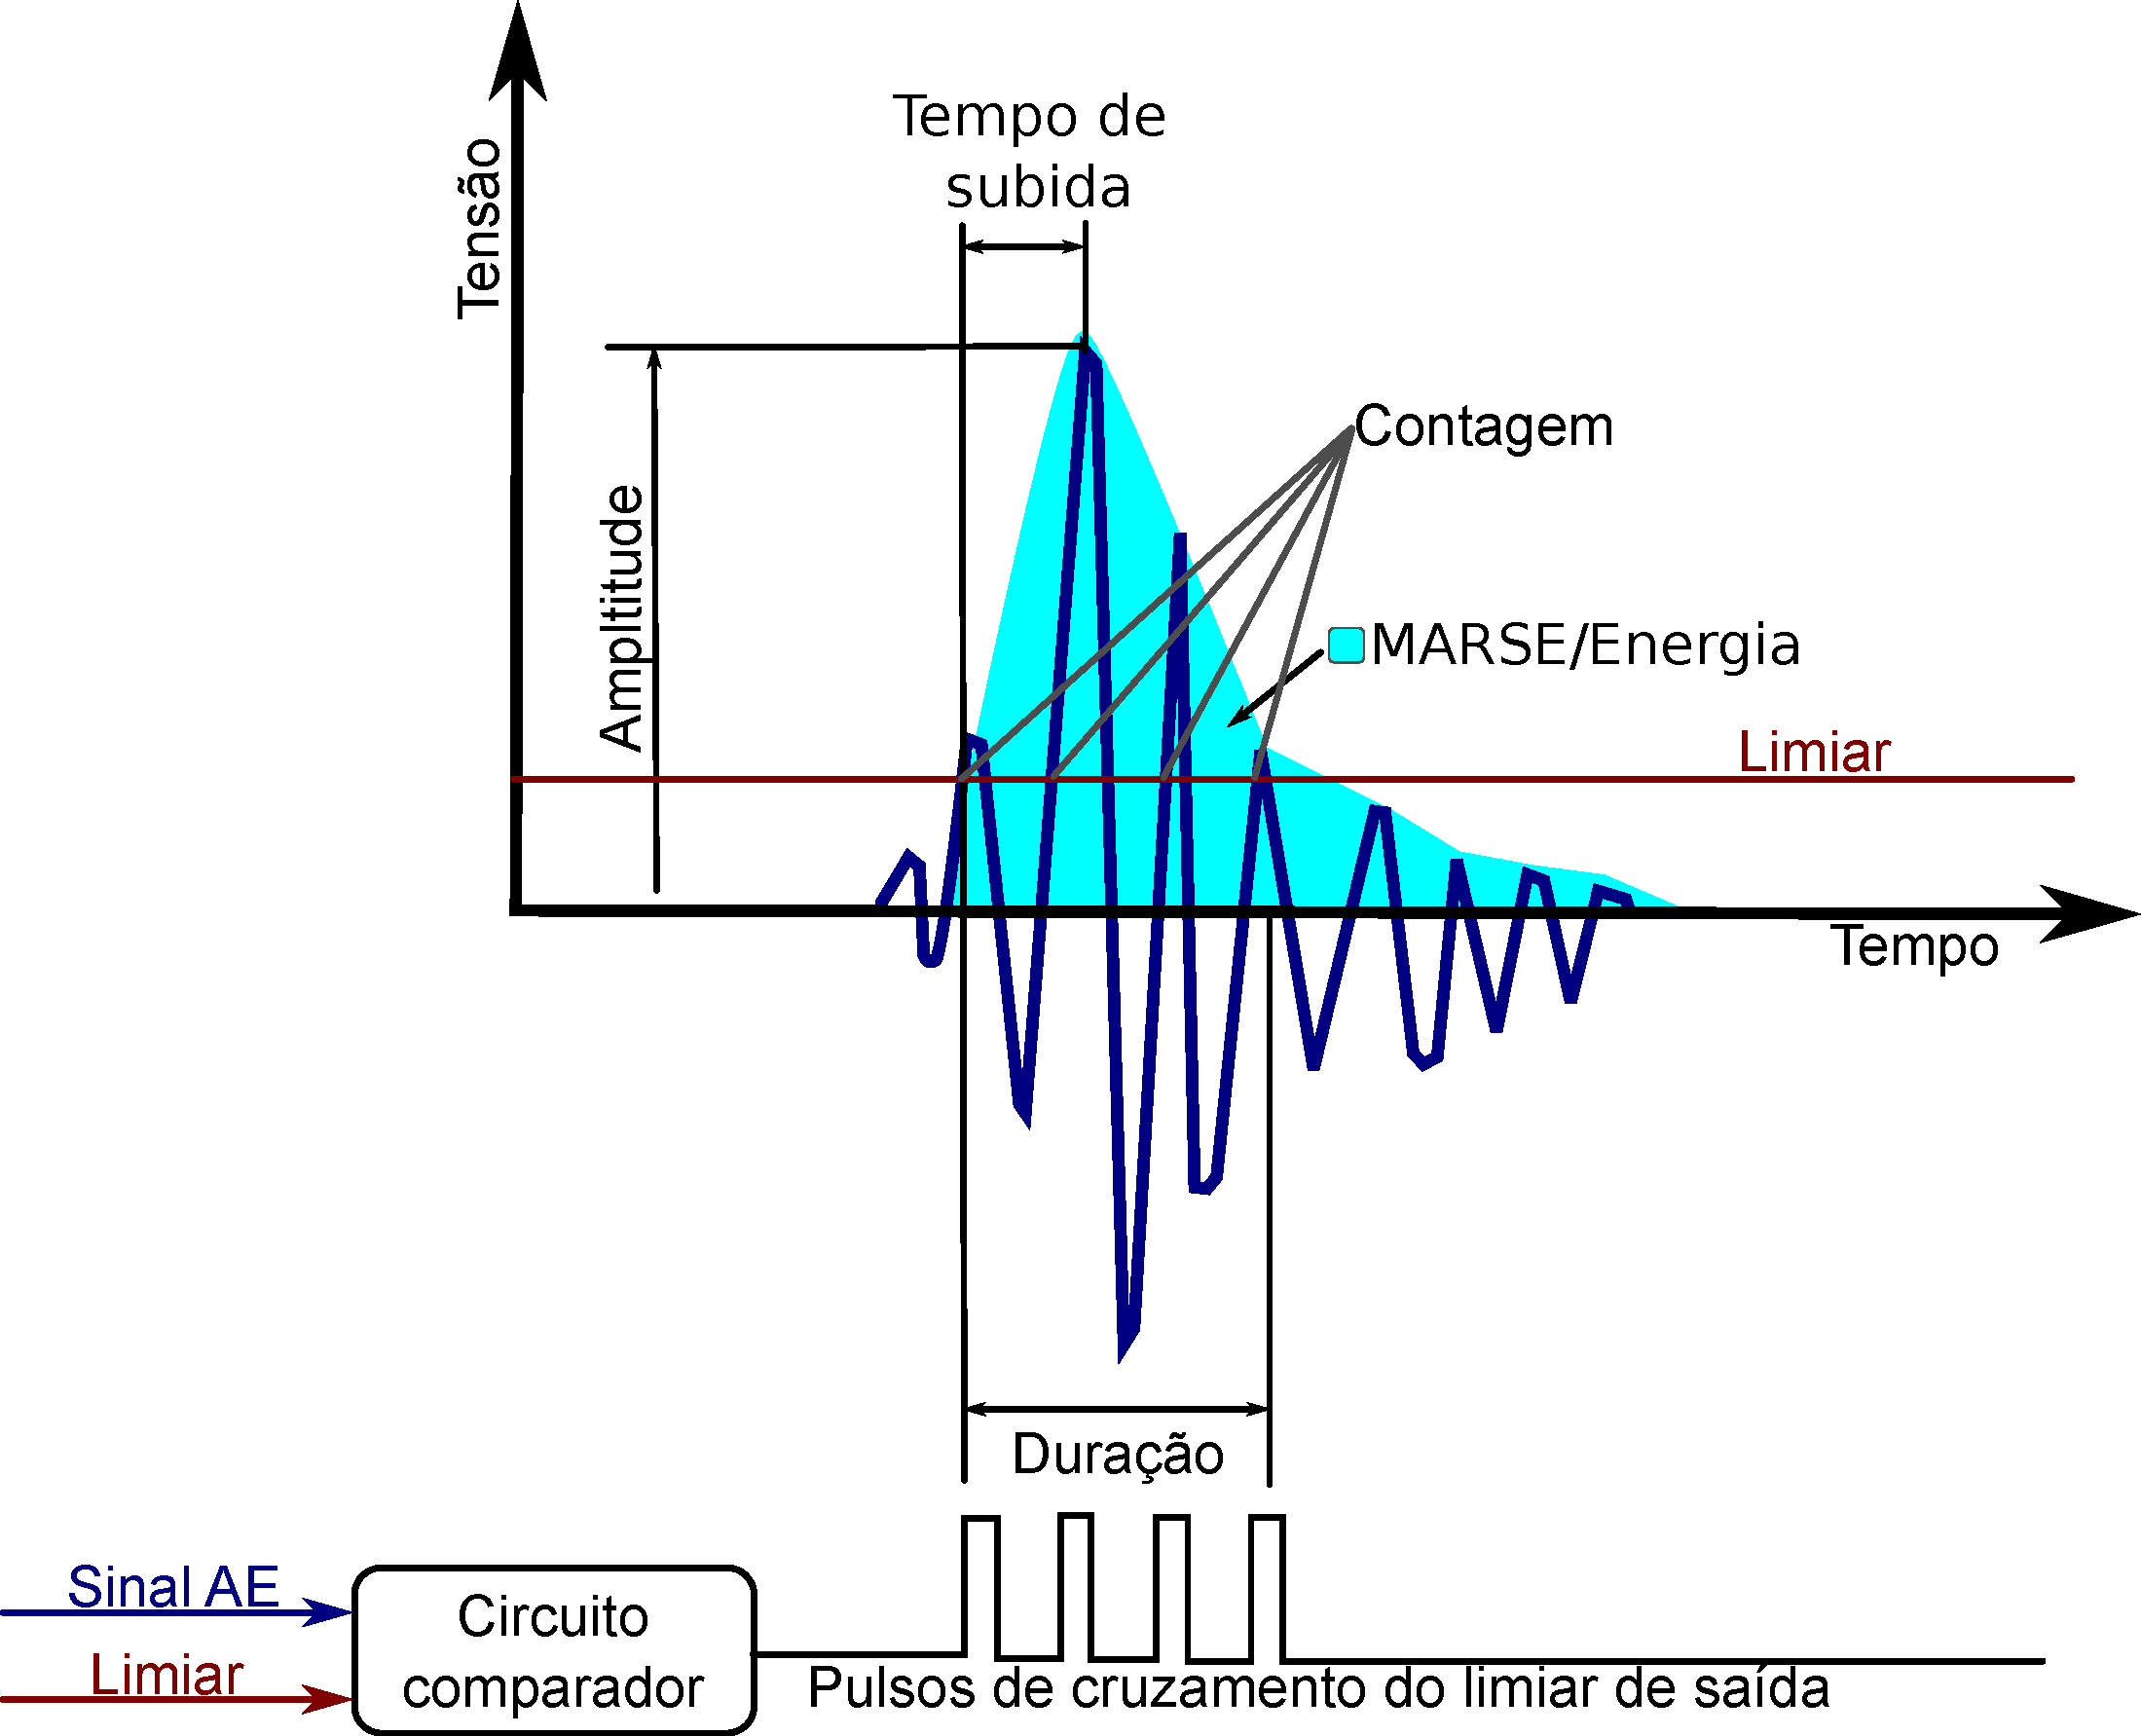
\includegraphics[width=.65\linewidth]{figs/Artigos/nde-ed-org/Figura2.pdf}
    \caption{Parâmetros de um \textit{hit} de EA: amplitude, tempo de subida, duração, contagens e energia (MARSE). Adaptado de \citeonline{nde-ed-ae-equipment}.}
    \label{fig:nde-ed-org-Fig2}
\end{figure}

A energia não tem definição única na literatura. Alguns autores usam a MARSE (\textit{measured area under the rectified signal envelope}, área medida sob o envelope retificado do sinal); outros, a soma dos quadrados do sinal, proporcional à energia elétrica do evento \cite{nde-ed-ae-equipment,liu2023review}. Este trabalho adota a forma quadrática, que é também a do sistema comercial usado como referência (Seção~\ref{sec:fund_hits}). Nem toda EA indica falha: atrito, vazamentos e o próprio escoamento geram sinais semelhantes, chamados de pseudo-fontes, e por isso os parâmetros dos \textit{hits} costumam ser interpretados em conjunto, ao longo do tempo, e não individualmente \cite{grosse2008acoustic}.

\subsection{Detecção de cavitação e trabalhos relacionados}

\citeonline{liu2023review} revisam a detecção de cavitação em bombas por vibração, EA, ruído e pulsação de pressão. Os métodos seguem um fluxo comum (Figura~\ref{fig:LiuFig1}): aquisição, processamento nos domínios do tempo, da frequência ou do tempo-frequência, extração de atributos e reconhecimento do estado por algoritmos de Inteligência Artificial (IA). A EA destaca-se na detecção incipiente, por operar em altas frequências, nas quais os transientes do colapso de bolhas têm relação sinal-ruído elevada \cite{Neill1997Detection,Alfayez2005}.

\begin{figure}[htbp]
    \centering
    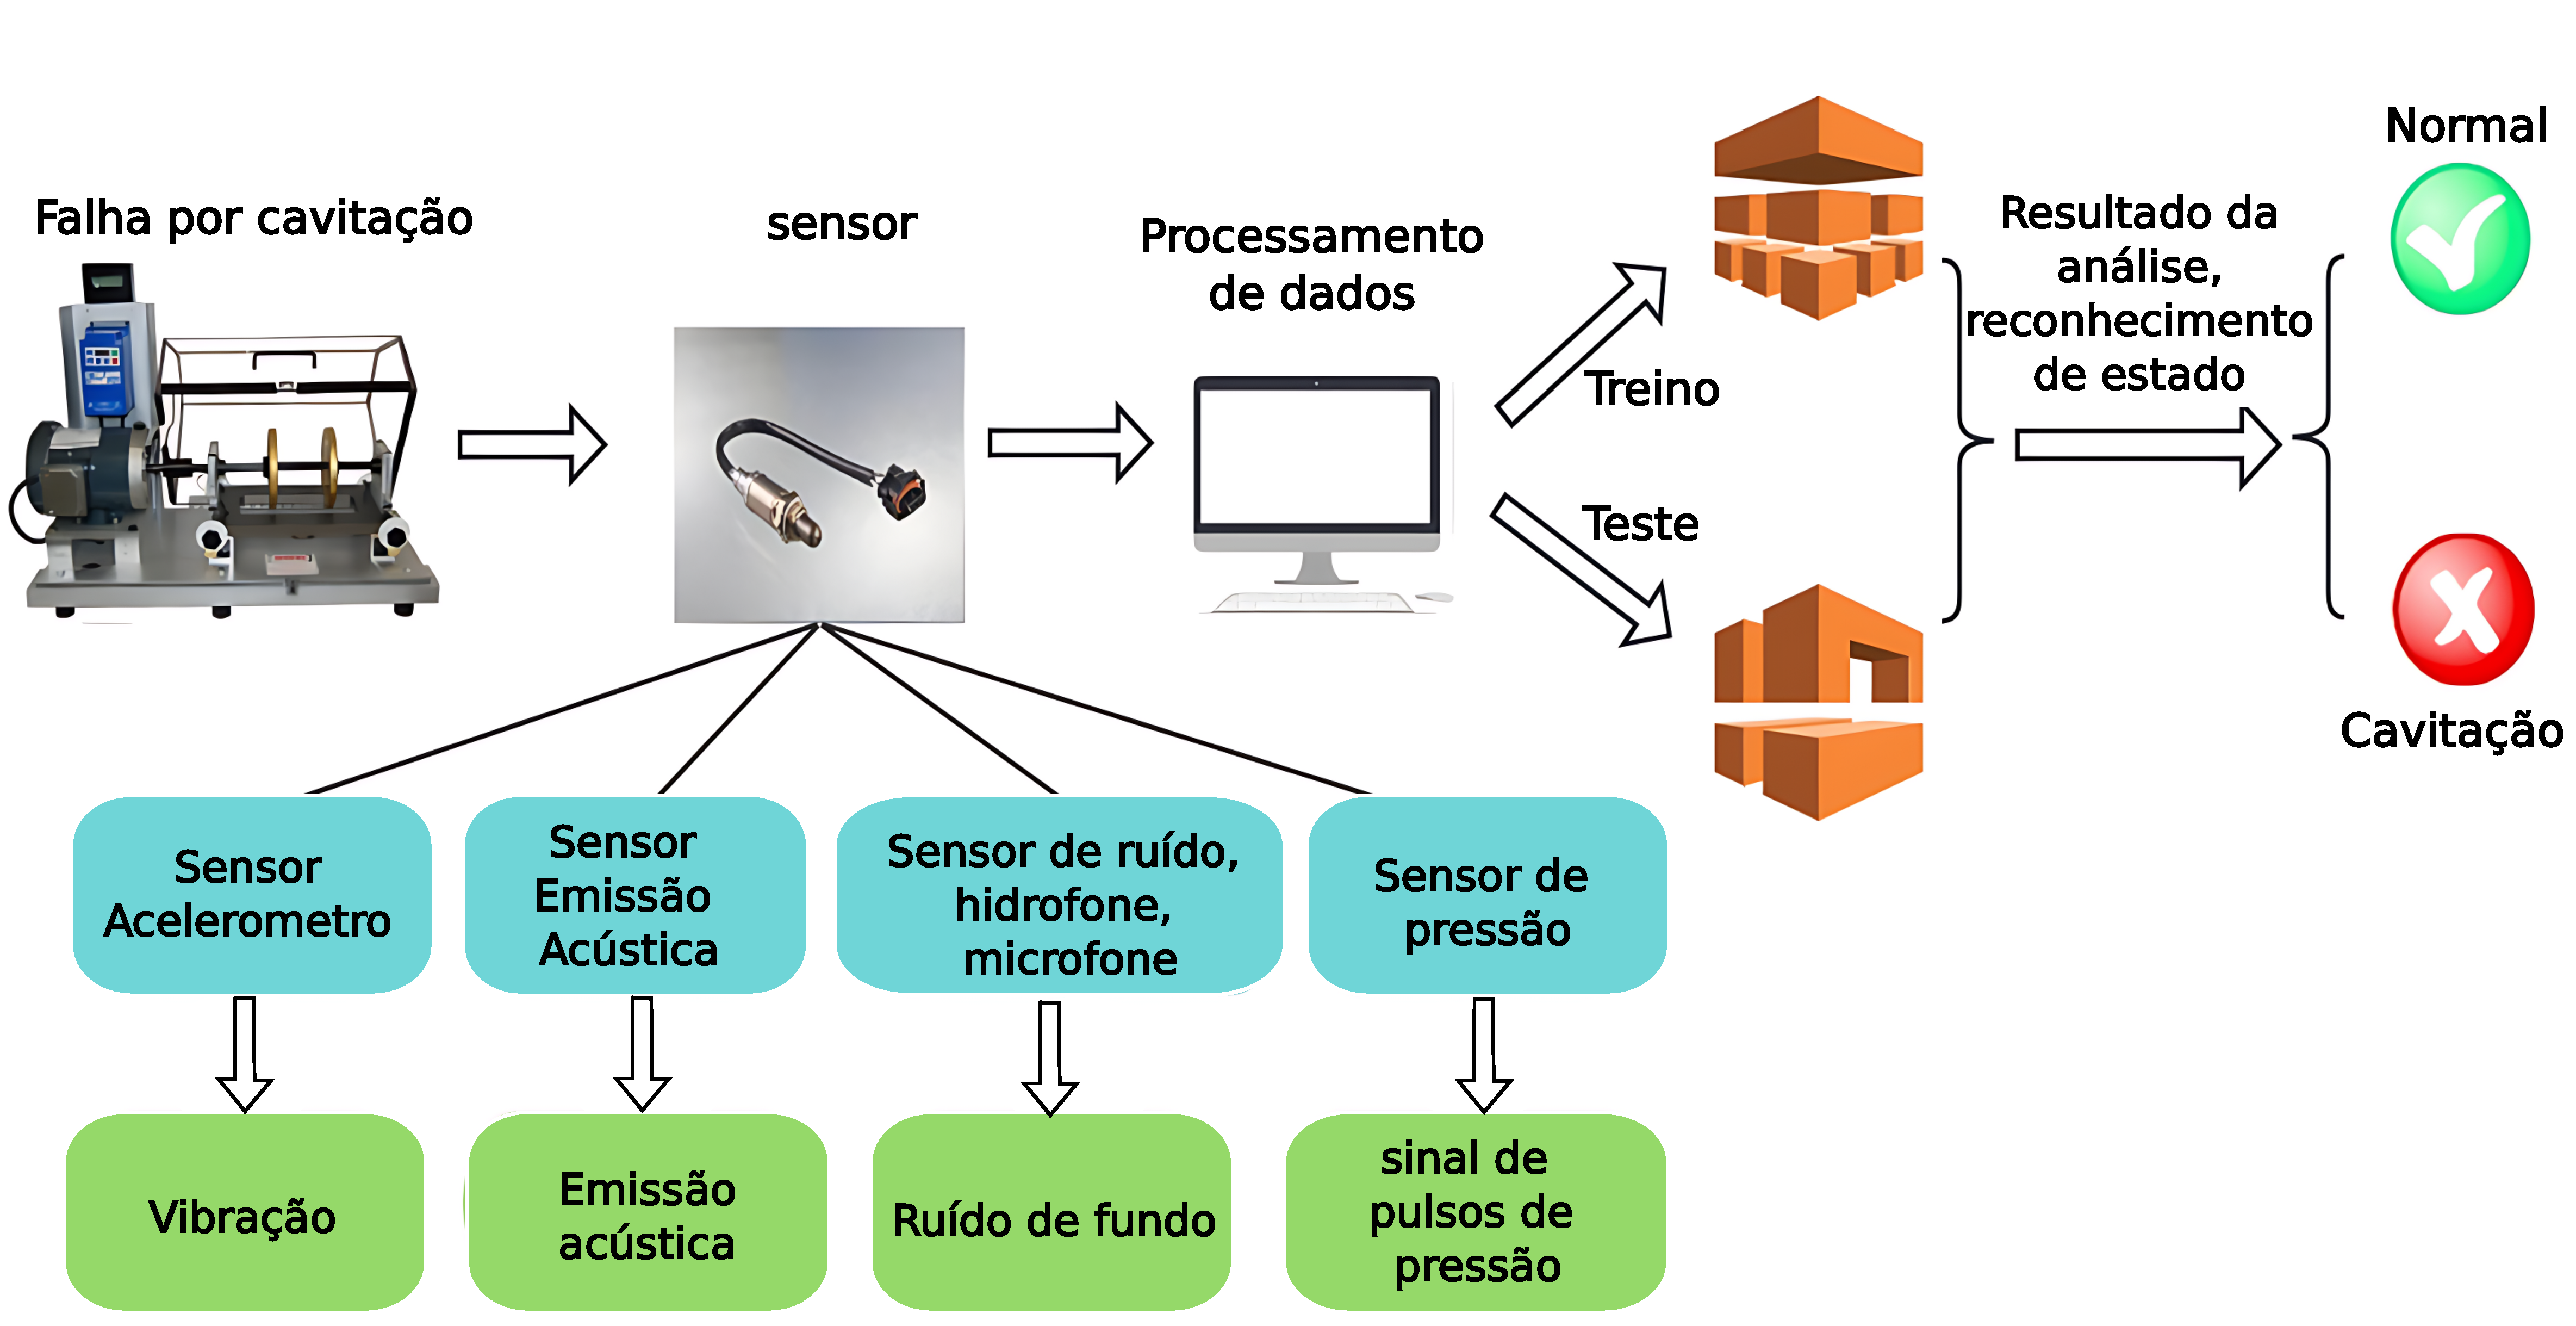
\includegraphics[width=.95\linewidth]{figs/Artigos/Liu/Figura1.pdf}
    \caption{Fluxo básico de detecção de cavitação com base em diferentes sinais. Adaptado de \citeonline{liu2023review}.}
    \label{fig:LiuFig1}
\end{figure}

A Tabela~\ref{tab:sintese_literatura_unificada} resume os trabalhos mais próximos deste, com os resultados relatados. A revisão não aponta um modelo superior de modo absoluto: o desempenho depende do sinal, do delineamento experimental e da validação adotada.

\begin{table}[htbp]
	\footnotesize
	\centering
	\caption{Síntese da literatura: sinais, atributos, modelos e resultados relatados, com destaque para implementações em FPGA.}
	\label{tab:sintese_literatura_unificada}
	\renewcommand{\arraystretch}{1.2}
	\resizebox{\textwidth}{!}{%
		\begin{tabular}{p{2.6cm} p{2.0cm} p{3.6cm} p{3.4cm} p{4.0cm} p{2.6cm}}
			\hline
			\textbf{Alvo} & \textbf{Sinal} & \textbf{Atributos} & \textbf{Modelo / implementação} & \textbf{Resultados relatados} & \textbf{Referências} \\ \hline
			\multicolumn{6}{l}{\textit{Estratégias gerais de detecção de cavitação}} \\ \hline
			Cavitação em bombas & Vibração & RMS, curtose, fator de crista, \textit{cepstrum} & SVM, \textit{Random Forest}, LSTM, CNN & Eficaz em cavitação moderada a severa; menos sensível à incipiente & \citeonline{liu2023review} \\ \hline
			Cavitação em bombas & EA & Amplitude, RMS, energia, contagens & Parâmetros e limiares & Detecção incipiente antes da queda de desempenho & \citeonline{Neill1997Detection,Alfayez2005,Alfayez2005ndt} \\ \hline
			Mancais hidrodinâmicos & EA e vibração & RMS, energia, contagens, tempo-frequência & Comparação e classificação & EA mais sensível nos estágios iniciais & \citeonline{poddar2021classification} \\ \hline
			Cavitação em turbinas & Acústico & Atributos espectrais & \(k\)-NN e GMM & 100\,\% (estático); \(>\)95\,\% (dinâmico) & \citeonline{amini2022development} \\ \hline
			\multicolumn{6}{l}{\textit{Aplicações com implementação em FPGA}} \\ \hline
			Rolamentos & EA & Atributos de EA em taxa ultrassônica & Multinúcleo em FPGA & Diagnóstico em tempo real & \citeonline{kang2015} \\ \hline
			Motores de indução & Corrente & Descritores estatísticos & MLP em FPGA & Precisão de 93,18\,\% & \citeonline{garcia2025detection} \\ \hline
			Qualidade de energia & Tensão & Parâmetros temporais e espectrais & MLP em Artix-7 & Classificação em tempo real & \citeonline{gaona2025fpga} \\ \hline
			Sistemas automotivos & Diversos & Características temporais & MLP em Zynq & Latência \(<\)1\,\(\mu\)s & \citeonline{shreejith2016} \\ \hline
			Rolamentos & Vibração & Envelope e estatísticas & MLP em Zynq-7000 & 95\,\% (tipo) e 89\,\% (severidade), base CWRU & \citeonline{toumi2022fpga} \\ \hline
			\textbf{Este trabalho} & \textbf{EA} & \textbf{Descritores de \textit{hits} por janela} & \textbf{MLP int8 em MicroBlaze ou IP HLS} & \textbf{Ver Capítulo~\ref{chap:resultados}} & --- \\ \hline
	\end{tabular}}
\end{table}

Este trabalho difere dos anteriores em três pontos. A redução de dados é feita na própria lógica, por detecção de \textit{hits} de EA a 10\,MSa/s, e não sobre sinais de baixa taxa. O classificador recebe estatísticas de populações de \textit{hits}, e não atributos de um sinal contínuo, de modo que o fluxo de dados acompanha a atividade acústica, e não a taxa de amostragem. E a avaliação separa as unidades físicas independentes (corridas, sessões ou rolamentos), o que, como se mostra no Capítulo~\ref{chap:resultados}, muda as conclusões em relação às acurácias usualmente relatadas. Os ensaios do MOMEA usam apenas EA; sinais de vibração aparecem só na validação externa com a base CWRU.
